\documentclass[conference]{IEEEtran}
\usepackage{graphicx,booktabs,amsmath,amssymb,array,url,hyperref,float}
\hypersetup{hidelinks}
\graphicspath{{figures/}}
\newcommand{\figwide}[3]{\begin{figure*}[!t]\centering\includegraphics[width=#2\textwidth]{#1}\caption{#3}\end{figure*}}
\newcommand{\figcol}[3]{\begin{figure}[!t]\centering\includegraphics[width=#2\columnwidth]{#1}\caption{#3}\end{figure}}
\title{Evidence-Grounded Clinical Trial Eligibility Screening with Qwen2.5, Low-Rank Adaptation, KV-Cached Decoding, Tiled Attention, and Speculative Generation}
\author{\IEEEauthorblockN{Fatima Shakir (23I-0503)}\IEEEauthorblockA{School of Computing, FAST National University of Computer and Emerging Sciences\\Islamabad Campus, Pakistan}}
\begin{document}\maketitle
\begin{abstract}
This study implements an educational clinical-trial eligibility screening prototype based on the TrialGPT Criterion Annotations dataset. A Qwen2.5-0.5B-Instruct decoder is adapted with low-rank fine-tuning to predict six expert eligibility categories and supporting patient-sentence identifiers. Patient-grouped splitting (37/8/8 patients) prevents patient-level overlap. On 206 held-out test annotations, classification accuracy is 67.48\%, macro-F1 is 0.3342, and evidence micro-F1 is 0.4706. Separate efficiency experiments compare explicit key/value (KV) caching, online-softmax tiled attention, and a custom greedy speculative decoder. The cache benchmark achieves a mean 1.13$\times$ speedup on a Tesla T4, whereas speculative decoding slows inference to 0.232$\times$ target-only speed because of low draft acceptance. A local CPU Gradio application supports criterion-level inspection and downloadable reports. Incorrect exclusion predictions and unsupported evidence demonstrate why the prototype cannot be used to make clinical enrollment decisions.
\end{abstract}
\begin{IEEEkeywords}clinical trial eligibility, TrialGPT, Qwen2.5, LoRA, evidence attribution, KV cache, online softmax, speculative decoding, Gradio\end{IEEEkeywords}
\section{Introduction}
Clinical-trial recruitment depends on matching free-text patient histories to heterogeneous inclusion and exclusion criteria. The challenge is not merely binary text classification: a system must distinguish affirmative eligibility, disqualification, non-applicability, and insufficient information, while grounding decisions in specific patient sentences. The TrialGPT benchmark makes these subtasks measurable through expert labels and sentence identifiers \cite{trialgpt}. Large language models can format judgments fluently but may invent support or infer the absence of a contraindication from missing documentation. This paper therefore evaluates both classification and evidence retrieval.
The project addresses six assignment tasks: model research and supervised adaptation; criterion-level classification and evidence verification; cache-aware greedy decoding; tiled online-softmax attention; greedy speculative decoding; and an independently accessible browser application. Efficiency experiments are not assumed to improve speed: correctness and measured trade-offs are reported separately. The application is educational and its aggregate patient outcome is a rule-based interpretation of predictions, not a patient-level ground truth label.
\section{Research Context and Prior Work}
Transformer self-attention provides contextual token representations but conventional full attention materializes a quadratic score matrix \cite{attention}. Qwen2.5 is an open-weight decoder family suitable for structured instruction following \cite{qwen}. LoRA constrains adaptation to low-rank weight updates, substantially reducing the number of trainable parameters \cite{lora}. TrialGPT motivates criterion-wise clinical reasoning with evidence rather than ungrounded patient-level labels \cite{trialgpt}. FlashAttention and online-softmax methods improve attention memory behavior through tiling and stable streaming normalization \cite{flash,online}. KV caching reuses attention states from earlier decoding steps; speculative decoding proposes multiple tokens with a draft model and verifies them with the target \cite{speculative}. Unlike claims of guaranteed acceleration, these methods can regress on short outputs, weak drafts, or Python-level implementations.

\section{Research Questions and Design Rationale}
The experimental study separates three questions that are often conflated. First, can supervised adaptation make a compact language model obey a strict six-label, evidence-grounded output contract? Second, when the predicted label is correct, is the cited sentence set also supported by expert annotation? Third, can computational improvements preserve generated tokens while reducing runtime or memory? A good classification score alone cannot answer the second question, and a faster decoder cannot repair the first two.

\subsection{Why criterion-level rather than patient-level supervision}
The benchmark supplies annotations for individual criterion--patient pairs. Consequently, the unit of evaluation is an annotation, not a complete trial-enrollment decision. For inclusion criteria, \texttt{included} means that the evidence supports satisfying that particular requirement. For exclusion criteria, \texttt{excluded} indicates that the disqualifying condition applies. These meanings must not be collapsed into a shared binary ``positive'' class. Missing documentation may produce \texttt{not enough information}; \texttt{not applicable} has a distinct meaning and occurs even among inclusion examples. The application aggregates multiple criterion predictions only as an explicit heuristic.

\subsection{Selection trade-offs}
The 0.5B model was chosen over the 1.5B alternative because the research budget included a Tesla T4 for training and a 16-GB-RAM, CPU-only Windows laptop for the final interactive application. A larger model might improve semantic reasoning, but no controlled 1.5B fine-tuning result was recorded; asserting an accuracy advantage would be speculative. The smaller target also allowed controlled decoding experiments to be run repeatedly. LoRA was preferred to updating all weights because it retains the pretrained checkpoint and stores a compact adapter. This reduces trainable optimizer state, although inference still needs the base model weights.

\subsection{Scope of evidence and claims}
The work demonstrates software engineering and measured benchmark behavior, not clinical efficacy. The dataset is small at the patient level and contains highly imbalanced criterion labels. There is no prospective patient recruitment study or clinician safety validation. All reported improvements are tied to the specific split, parsing rules, hardware, and output schema.

\section{Model Selection and Architecture}
Two feasible Apache-2.0 Qwen2.5 candidates were considered: 0.5B (approximately 494 million parameters, 0.92 GiB FP16 weights) and 1.5B (approximately 1.54 billion parameters, 2.87 GiB FP16 weights). Both are decoder-only models with grouped-query attention and a nominal 32,768-token context in the recorded comparison table. The 0.5B variant was selected for Tesla T4 fine-tuning and CPU deployment on a 16-GB-RAM laptop. The 1.5B model was an alternative, \emph{not} a separately fine-tuned model in this submission. The selected model has 24 transformer layers. A 12-layer draft model was initialized from alternating target layers, producing 315,084,160 parameters (63.78\% of the target). Model availability does not establish clinical suitability.
\begin{figure}[!t]\centering\fbox{\begin{minipage}{0.94\columnwidth}\centering\small Patient record + criterion type + criterion text\\$\downarrow$\\Sentence numbering and prompt assembly\\$\downarrow$\\Qwen2.5-0.5B decoder + LoRA $\Delta W=BA$\\$\downarrow$\\Greedy JSON generation: label, evidence\_ids\\$\downarrow$\\Evidence ID validation + citation extraction\\$\downarrow$\\Criterion table, preliminary aggregation, CSV/JSON export\end{minipage}}\caption{End-to-end educational screening workflow. Evidence selection is model-generated and requires verification.}\end{figure}

\section{Dataset Integrity and Split Protocol}
The prescribed NCBI TrialGPT Criterion Annotations dataset contains 1,015 original records from 53 patients. One record has a missing criterion text; the cleaned training partition contains 602 examples, while validation and test contain 206 each, totaling 1,014 usable records. Unique patient IDs were sorted and shuffled using NumPy \texttt{default\_rng(42)}, with 37 patients assigned to training, eight to validation, and eight to test. All annotations from a patient remain within one partition. The manifest must be distributed with the reproducibility files. Earlier model predictions and explanations contained in the dataset were not used as model input. Test data were reserved for the final held-out evaluation.
\begin{table}[!t]\centering\caption{Patient-grouped data partition}\begin{tabular}{lrr}\toprule Partition&Patients&Usable annotations\\\midrule Training&37&602\\Validation&8&206\\Held-out test&8&206\\\midrule Total&53&1,014\\\bottomrule\end{tabular}\end{table}
\section{Prompt and Supervision}
Each example combines the numbered patient description, criterion type (inclusion or exclusion), criterion text, and an \texttt{Answer:} suffix. The response is a JSON object with exactly \texttt{label} and \texttt{evidence\_ids}. Six labels are retained: \texttt{included}, \texttt{not included}, \texttt{excluded}, \texttt{not excluded}, \texttt{not applicable}, and \texttt{not enough information}. Importantly, \texttt{not applicable} also occurs in inclusion criteria; filtering it by criterion type would be incorrect. Evidence IDs must exist in the patient record. An empty list does not automatically imply eligibility. For long inputs, tokenizer truncation is limited to 1,024 tokens. Recorded token lengths: training median 230, 95th percentile 420, maximum 549; validation median 271, maximum 383. Thus the recorded training and validation prompts do not exceed 1,024 tokens, though arbitrary application inputs still need length validation.

\section{Reproducible Data Preparation and Leakage Controls}
The split protocol is deterministic: collect unique patient identifiers, sort them, shuffle with NumPy's \texttt{default\_rng(42)}, and allocate 37, 8 and 8 patients. Grouping is necessary because several criteria share the same patient's narrative. A random annotation-level split could allow the model to see substantially the same patient record during training and testing, inflating measured generalization. A leakage check verifies that the patient-ID intersections across train, validation and test are empty.

One missing criterion text was identified in the raw collection and excluded from usable supervision, leaving 1,014 examples. The removal affects the training count; validation and test retain 206 annotations each. The manifest should preserve the original patient IDs, split assignments and record counts so that future runs can reconstruct the exact partition. The test partition was reserved for the final evaluation; intermediate tuning used validation.

Patient descriptions were transformed into a sequence of explicitly numbered sentences. Evidence supervision refers to those sentence IDs rather than to character offsets. The text normalization must be deterministic: a citation ID is meaningful only when it maps back to the identical sentence shown to the model. An application that renumbers sentences differently from the training pipeline risks displaying apparently valid but semantically wrong citations.

\subsection{Label distribution and interpretation}
The six categories are not interchangeable. In the held-out set, \texttt{not excluded} (91 records) and \texttt{not enough information} (66 records) dominate, while \texttt{not included} has seven and \texttt{excluded} has no gold examples. Thus a model that over-predicts a majority class may obtain reasonable accuracy while failing precisely the minority decisions that matter most for patient safety. Per-class support, recall and confusion matrices are therefore required, rather than optional, diagnostics.

\subsection{Input length and evidence preservation}
The 1,024-token input cap was selected after measuring the training and validation token distributions. Their observed maxima, 549 and 383 tokens respectively, were below that limit. This establishes that those measured prompts were not truncated at 1,024 tokens; it does not establish that arbitrary unseen clinical narratives fit. In production-like use, an overlength input should trigger explicit validation or careful segmentation. Silently dropping late sentences could remove the only supporting evidence and make an apparently confident answer ungrounded.

\section{Parameter-Efficient Training}
Qwen2.5-0.5B-Instruct was adapted using LoRA rank $r=8$, $\alpha=16$ on query/value projections, with 540,672 trainable parameters (0.1093\% of approximately 494 million). The learning rate was $2\times10^{-4}$, effective batch size eight, and training used a Tesla T4 with 14.56 GiB GPU memory. The saved training summary reports three epochs and 252.28 seconds total training. Intermediate logged checkpoints include epoch-1 train/validation losses 0.1581/0.168451 and epoch-2 losses 0.1091/0.144346. The best recorded validation loss was 0.1443456 at step 225. The final aggregate training loss in the saved summary (0.26158) is not the same statistic as the plotted checkpoint losses; these should not be conflated.
\figcol{training_loss.png}{1.0}{Saved training-loss figure from the submitted experiments. Training and validation trends are interpreted as optimization diagnostics, not proof of clinical generalization.}

\section{Training Objective, Decoding Contract, and Reproducibility}
For a tokenized training pair $(x,y)$, supervised causal fine-tuning minimizes the negative log-likelihood of the target answer tokens conditioned on the input:
\begin{equation}
\mathcal{L}_{\rm SFT}=-\sum_{t=1}^{|y|}\log p_{\theta,\Delta}(y_t\mid x,y_{<t}).
\end{equation}
Here $\theta$ denotes frozen pretrained weights and $\Delta$ the trainable low-rank updates. For a projection matrix $W\in\mathbb{R}^{d_{\rm out}\times d_{\rm in}}$, LoRA uses
\begin{equation}
W'=W+\frac{\alpha}{r}BA,\quad
A\in\mathbb{R}^{r\times d_{\rm in}},\;
B\in\mathbb{R}^{d_{\rm out}\times r}.
\end{equation}
With $r=8$ and $\alpha=16$, the adapter updates only query and value projections. This explains the recorded 540,672 trainable parameters, a small fraction of the approximately 494 million total.

The training prompt deliberately uses a plain-text format rather than relying on a separately applied chat template. It starts with an educational screening instruction, provides a numbered patient description, states the criterion type and criterion text, and ends in \texttt{Answer:}. The desired completion is a JSON object with exactly \texttt{label} and \texttt{evidence\_ids}. During deterministic evaluation, greedy decoding reduces sampling variability, but it does not guarantee valid JSON or correct semantics. Both syntax validity and sentence-ID membership must be checked after generation.

\subsection{Reported optimization behavior}
The training run used 225 optimization steps and approximately 252 seconds on a Tesla T4. The checkpoint logs show declining training loss and a validation loss of approximately 0.1443 at the selected checkpoint. These curves are consistent with adaptation to the supervised format; they do not demonstrate calibration or reliable recognition of all labels. In particular, rare-class failures in the held-out test remain severe despite a successful optimization run.

\subsection{Baseline fairness}
The before/after comparison uses the same base architecture and the same strict parser. The base model's zero score is attributable to all 206 baseline validation outputs failing the structured-output contract, rather than evidence that the base model cannot understand clinical text. The fine-tuned model's zero invalid outputs is therefore an important improvement in interface compliance. A future comparison could add constrained JSON decoding for both checkpoints to separate semantic improvement from format compliance, but no such additional result is claimed here.

\section{Evaluation Definitions}
Classification accuracy is the fraction of exact label matches; macro-F1 averages per-class F1 to expose minority-class failures. Evidence precision, recall and F1 compare predicted and expert sentence-ID sets. With $TP$, $FP$, and $FN$ aggregated over examples, $P=TP/(TP+FP)$, $R=TP/(TP+FN)$, and $F_1=2PR/(P+R)$. Empty-gold/empty-predicted cases require an explicit convention. The held-out results report strict macro evidence F1 (empty/empty treated as zero) and an alternative empty/empty-as-one score, because the latter can appear deceptively high when evidence is frequently absent. Confusion matrices and per-class support are provided to avoid hiding skewed labels behind overall accuracy.

\section{Validation: Before and After Adaptation}
The unadapted Qwen baseline produced 206 invalid parsed outputs on the validation set, yielding 0.0 accuracy and macro-F1 under the strict structured-output evaluator. This does \emph{not} imply zero general language understanding; it measures failure to meet the requested JSON/label contract. The fine-tuned model produced zero invalid outputs and achieved 72.82\% validation accuracy and 0.3846 macro-F1. Inclusion and exclusion subset accuracies were 74.24\% and 72.14\%, respectively. Validation evidence micro precision/recall/F1 were 0.6087/0.3652/0.4565; exact evidence-set agreement was 0.6602. These are validation measurements, not held-out test results.
\begin{table}[!t]\centering\caption{Validation comparison on 206 annotations}\begin{tabular}{lrrr}\toprule Model&Accuracy&Macro-F1&Invalid\\\midrule Base 0.5B&0.000&0.000&206\\Fine-tuned LoRA&0.7282&0.3846&0\\\bottomrule\end{tabular}\end{table}
\figcol{confusion_matrix_overall.png}{1.0}{Saved validation confusion matrix. Strong majority-class performance does not imply reliable rare-category discrimination.}

\section{Held-Out Test Classification Results}
On eight unseen patients (206 annotations), the fine-tuned model attained accuracy 0.674757 (139/206), macro-F1 0.334168 and zero invalid outputs. Support varies substantially: \texttt{not excluded} has 91 examples, \texttt{not enough information} 66, \texttt{included} 27, \texttt{not applicable} 15, \texttt{not included} seven, and \texttt{excluded} zero. No test-set recall can be estimated for a class with zero gold support. The model recalled all 91 \texttt{not excluded} examples but achieved zero recall on the seven \texttt{not included} and 15 \texttt{not applicable} cases. These patterns explain why the macro-F1 is much lower than accuracy.
\begin{table}[!t]\centering\caption{Held-out test per-class results}\scriptsize\begin{tabular}{lrrrr}\toprule Label&P&R&F1&N\\\midrule included&.606&.741&.667&27\\not included&0&0&0&7\\excluded&0&0&0&0\\not excluded&.695&1.000&.820&91\\not applicable&0&0&0&15\\not enough info.&.667&.424&.519&66\\\midrule Macro average&.328&.361&.334&206\\\bottomrule\end{tabular}\end{table}
\figcol{final_test_confusion_overall.png}{1.0}{Held-out test confusion matrix from saved evaluation outputs.}
\section{Inclusion and Exclusion Diagnostics}
Inclusion and exclusion criteria require different interpretations: inclusion \texttt{included} indicates satisfaction, while exclusion \texttt{excluded} indicates a disqualifying condition. The split-specific confusion matrices expose confusion among insufficient-information, applicability and negative labels. These are not equivalent to a patient-level enrollment classifier; the application derives only a preliminary aggregate verdict. Rare labels cannot be made reliable by an overall accuracy threshold alone. Explicit uncertainty and citation checking remain essential.
\figcol{final_test_confusion_inclusion.png}{1.0}{Held-out inclusion confusion matrix.}
\figcol{final_test_confusion_exclusion.png}{1.0}{Held-out exclusion confusion matrix.}


\section{Quantitative Interpretation of Classification Errors}
The validation accuracy of 72.82\% and held-out test accuracy of 67.48\% are computed on different patient groups; their difference should not be interpreted as a statistically established generalization gap from only eight patients per split. On the test set, 139 of 206 criterion labels match expert labels, leaving 67 errors. Macro-F1 of 0.3342 is much lower than accuracy because performance varies sharply by class.

The \texttt{not excluded} class has recall 1.000 over 91 gold examples, yet this is not sufficient evidence of robust exclusion handling: predicting \texttt{not excluded} too frequently also causes errors when a criterion is applicable or the patient record is incomplete. The \texttt{not included} class has seven gold examples and zero recall; \texttt{not applicable} has 15 and zero recall. The absence of gold \texttt{excluded} examples prevents estimation of held-out exclusion recall. The observed metformin failure in the local demonstration is therefore an informative stress test, but not a substitute for a properly supported test-set estimate.

\subsection{A taxonomy of observed failures}
The saved error review records 67 classification mismatches, 53 evidence mismatches, and 23 cases in which both were wrong. These counts overlap and must not be added as though they represented disjoint groups. Several failure mechanisms are distinguishable. \emph{Category confusion} occurs when insufficient information is converted into a definite positive or negative label. \emph{Applicability confusion} occurs when a criterion that does not apply is treated as satisfied. \emph{Citation drift} occurs when a model selects an existing but irrelevant sentence ID. Finally, \emph{error propagation} occurs when the application aggregates an incorrect criterion label into a misleading patient-level summary.

For example, the recorded shock/ARDS-related case 185 included clinically relevant signs such as tachypnea, tachycardia and hypotension, but the model predicted insufficient information and selected unrelated arm-pain evidence. In case 422, a birth-control inclusion requirement annotated as not applicable was predicted included with age-related evidence. These are different errors: the first misses clinical relevance, while the second confuses applicability with satisfaction. The local metformin case combines a false negative exclusion decision with irrelevant evidence and a falsely reassuring aggregate outcome.

\subsection{Why not silently repair outputs}
A rule that replaces a model label whenever the words ``metformin'' and ``excluded'' co-occur would make the demonstration look correct without validating clinical semantics. It could fail on negation, historical medications, discontinued treatment, or conditional criteria. The safer engineering response is to show the unmodified model output, its evidence, and a review warning when support is missing or inconsistent. Such a warning is a user-interface safeguard, not a claim that the underlying prediction has been corrected.

\section{Evidence Retrieval Results}
Held-out evidence retrieval yielded $TP=40$, $FP=36$, $FN=54$, micro precision 0.5263, micro recall 0.4255, and micro-F1 0.4706. Strict macro-F1 was 0.1601; exact evidence-set match was 0.7427. However, 124 examples had both expert and predicted evidence empty. Assigning those cases F1=1 increases macro-F1 to 0.7620, whereas computing macro-F1 over nonempty-union cases gives 0.4021. Reporting all conventions avoids overstating grounding quality. Exact evidence agreement alone is insufficient to establish valid clinical reasoning.
\begin{table}[!t]\centering\caption{Held-out evidence metrics}\begin{tabular}{lr}\toprule Measure&Value\\\midrule Micro precision&0.5263\\Micro recall&0.4255\\Micro F1&0.4706\\Strict macro F1&0.1601\\Macro F1, empty/empty=1&0.7620\\Macro F1, nonempty union&0.4021\\Exact evidence-set match&0.7427\\Both sets empty&124/206\\\bottomrule\end{tabular}\end{table}

\section{Detailed Error Analysis}
The saved held-out error analysis records 67 classification errors, 53 evidence errors, and 23 examples where both were wrong. Case 185: a patient with tachypnea, tachycardia and blood pressure 80/60 was expert-labeled as satisfying a shock/ARDS-related inclusion criterion, yet the model returned insufficient information and cited unrelated arm pain. Case 422: a birth-control inclusion criterion was expert-labeled \texttt{not applicable}, but the model returned \texttt{included} and cited age rather than sexual-history evidence. Case 745 likewise illustrates uncertainty about applicability in a birth-control criterion. Other recorded failures involve insufficient clinical information and irrelevant sentence selection. The local demonstration provides a particularly transparent error: for a patient currently taking metformin, the exclusion criterion ``Patients currently taking metformin are excluded'' should produce \texttt{excluded} citing sentence 2, but the model returned \texttt{not excluded} citing the diabetes sentence 1. Both cached and uncached decoding reproduced this error. The rule-based preliminary outcome therefore misleadingly said that no disqualifying criterion was found. This is a model error propagated through an otherwise functioning interface, not evidence that the exclusion criterion was met.


\section{Evidence Metrics: What the Numbers Mean}
Evidence retrieval is a set-prediction task. For each criterion, the predicted set contains sentence identifiers selected by the model; the reference set contains expert-annotated identifiers. An identifier can be syntactically valid yet semantically unhelpful, so the set metric is a necessary but incomplete proxy for grounded reasoning.

The held-out aggregate counts are 40 true-positive, 36 false-positive and 54 false-negative sentence-ID decisions. These yield micro precision 0.5263 and micro recall 0.4255: among cited evidence IDs, only about 52.6\% match the expert evidence set, and the model retrieves about 42.6\% of expert evidence identifiers. Their harmonic mean is 0.4706. In applications, low recall can omit decisive contraindications, while low precision can attach misleading justification to a label.

\subsection{Empty-set conventions and score inflation}
In 124 of 206 held-out annotations, both predicted and expert evidence sets are empty. When empty/empty receives a perfect score, macro evidence F1 rises to 0.7620. Under a strict convention that assigns zero to empty/empty, macro F1 is 0.1601; restricting the average to cases where at least one set is nonempty yields 0.4021. These apparently contradictory values are different aggregation conventions, not inconsistent experiments. They should always be reported together with the definition and the count of empty/empty cases. The exact evidence-set match of 0.7427 is likewise influenced by the large number of jointly empty examples.

\subsection{Evidence validation in the application}
The application can check that generated IDs exist in the normalized patient sentence map, remove malformed references and display the corresponding original text. This prevents fabricated indices from being presented as real sentences. It cannot establish that the sentence logically entails the label. A valid ID such as the diabetes sentence cited for the metformin exclusion can still be wrong. Semantic verification and clinician oversight therefore remain unresolved research problems.

\section{KV-Cached Greedy Autoregression}
For ordinary greedy decoding, the next token is $x_t=\arg\max_v p(v\mid x_{<t})$. Without a cache, the model recomputes all previous-token keys and values at each step. Cache-aware decoding processes the prompt once (prefill), stores per-layer KV tensors, then passes only the newest token with its past state; attention masks and position handling must remain consistent. The custom notebook implementation was checked for token-level identity. Three Tesla T4 configurations (64/16, 128/32 and 256/64 prompt/output tokens), each with three repeats, produced speedups 1.0033$\times$, 1.2936$\times$ and 1.0929$\times$, respectively. Mean speedup was 1.1299$\times$ and mean measured peak-memory reduction 10.51\%. Cache overhead can offset savings for short generations.
\figcol{kv_cache_final_latency.png}{1.0}{Saved explicit cache-aware decoding latency comparison on Tesla T4.}
\figcol{kv_cache_final_memory.png}{1.0}{Saved cache experiment memory comparison; measured allocation depends on setup and sequence lengths.}
\section{Local CPU Decoding Demonstration}
The standalone Gradio interface provides two actual generation modes through \texttt{use\_cache=True/False}. These library-enabled modes are distinct from the explicit notebook cache implementation. On one three-criterion CPU demonstration, total measured generation time was 11.84 seconds cached versus 55.62 seconds uncached, or 4.70$\times$ speedup. Criterion-level cached/uncached times were 3.771/15.393, 3.575/18.936 and 4.494/21.293 seconds. Labels and evidence IDs matched across both modes. These single-run local timings should not be interpreted as repeated controlled performance estimates. The interface's live comparison can repeat measurements on a chosen criterion.


\section{Cache-Aware Decoding: Algorithm and Controls}
In autoregressive inference, every output token depends on the full preceding sequence. Recomputing all prior attention states at each step is wasteful. The explicit cached implementation separates \emph{prefill}, which processes the entire input prompt and builds layerwise key/value tensors, from \emph{decode}, which forwards the newest token while reusing the stored state. The uncached reference forwards the growing full sequence each step. Both paths use deterministic argmax selection, the same stopping condition and the same prompt.

For layer $\ell$, cache growth can be represented as
\begin{equation}
K^{(\ell)}_{1:t}=[K^{(\ell)}_{1:t-1};K^{(\ell)}_t],\qquad
V^{(\ell)}_{1:t}=[V^{(\ell)}_{1:t-1};V^{(\ell)}_t].
\end{equation}
The new query attends to cached positions and its own position under a causal mask. Position IDs or rotary position indices must reflect the full sequence offset; resetting them to zero at each decode step would break equivalence. Implementations must also avoid counting the initial prefill as though it were per-token decoding.

\subsection{Benchmark design and interpretation}
The saved GPU experiment tested prompt/output token lengths of 64/16, 128/32 and 256/64 with three repeats each. Its speedups were 1.0033, 1.2936 and 1.0929, averaging 1.1299; measured peak memory was reduced by approximately 10.51\% on average. The smallest case shows that caching need not help materially when prompt and generation are short. Speedup also varies with sequence length and measurement overhead.

The local CPU browser experiment is a separate environment and should not be pooled with the T4 measurements. For the three demonstration criteria, cached generation took 3.771, 3.575 and 4.494 seconds; uncached generation took 15.393, 18.936 and 21.293 seconds. Summing these measurements gives 11.84 versus 55.62 seconds, a 4.70-fold speedup for this one demonstration. Identical labels and evidence IDs were observed in both modes. The local UI modes use the model library's cache option; the notebook provides the separately required explicit cache-aware implementation.

\section{Tiled Attention and Online Softmax}
Reference scaled dot-product attention computes $\operatorname{softmax}(QK^\top/\sqrt{d}+M)V$. Tiling processes blocks of keys and values without retaining the entire $N\times N$ score matrix. The online normalizer updates running maximum $m$ and partition sum $\ell$ per query row: $m'=\max(m,m_{\rm tile})$, $\ell'=e^{m-m'}\ell+\sum_j e^{s_j-m'}$. Weighted outputs are rescaled consistently. Eighteen correctness cases passed on Tesla T4 with maximum absolute difference $9.54\times10^{-7}$ against the reference. The educational PyTorch-loop implementation was slower than fused PyTorch SDPA because of Python iteration and many small GPU launches; memory efficiency does not guarantee speed. The experiments used float32, sequence lengths 128, 256, 512, and tile sizes 32 and 64.
\figcol{attention_latency.png}{1.0}{Reference, tiled and optimized SDPA attention latency from saved benchmarks.}
\figcol{attention_memory.png}{1.0}{Saved attention memory measurements; resident-model memory affects measured peaks.}


\section{Online Softmax Derivation and Numerical Checks}
For each query row, ordinary attention calculates all logits $s_j=q^\top k_j/\sqrt{d}$, subtracts their maximum, exponentiates, normalizes and multiplies by values. A tiled implementation processes key/value blocks without storing all scores simultaneously. Let $m$ be the running maximum logit, $\ell$ the running sum of shifted exponentials, and $o$ the running unnormalized weighted value sum. For a new tile with maximum $m_b$, partition sum $\ell_b$ and weighted sum $o_b$, define
\begin{align}
m'&=\max(m,m_b),\\
\ell'&=e^{m-m'}\ell+e^{m_b-m'}\ell_b,\\
o'&=e^{m-m'}o+e^{m_b-m'}o_b.
\end{align}
After all tiles, the normalized output is $o/\ell$. Rescaling both the denominator and numerator is essential; otherwise later tiles receive the wrong relative weights. Causal masking must exclude future key positions before computing tile maxima and exponentials.

\subsection{Correctness versus performance}
The recorded implementation passed 18 controlled correctness cases with a maximum absolute error of $9.54\times10^{-7}$ relative to the reference. Tests included float32 calculations, multiple sequence lengths and tile sizes, and causal masking. This tolerance supports numerical equivalence for the tested cases; it is not a formal proof for every tensor shape or precision.

The PyTorch-loop tiled implementation ran slower than optimized fused scaled dot-product attention. This result is expected when many small Python-managed GPU operations and kernel launches replace a fused backend. Tiling addresses intermediate storage and data movement, but speed requires implementation-level fusion and favorable memory access patterns. The saved memory plots also reflect resident model and allocator behavior, so absolute peak differences should not be interpreted as isolated attention-matrix allocation alone.

\section{Custom Greedy Speculative Decoding}
Speculative decoding lets a smaller draft model propose $k$ candidate tokens and the target model verify them, accepting a matching prefix. On disagreement, the target token is emitted and cache state is corrected; greedy equivalence requires identical final tokens to target-only generation. The custom draft retained 12 of 24 Qwen layers, initialized from alternating target layers and distilled with LoRA using 100 teacher-generated examples over 75 steps (61.22 seconds). With $k=4$, all benchmark token-identity checks passed. Across three benchmark configurations, mean target latency was 1.0873 seconds, speculative latency 4.6851 seconds, mean speedup 0.2323$\times$, and draft acceptance 5.28\%. Mean peak GPU memory increased from 1.6311 to 1.7151 GiB. The draft is still 63.78\% of the target size; low token acceptance and Python overhead explain the slowdown. This is a valid negative performance result, not an acceleration claim.
\figcol{speculative_latency.png}{1.0}{Target-only versus custom speculative decoding latency.}
\figcol{speculative_acceptance.png}{1.0}{Draft acceptance statistics: low acceptance limits useful verification amortization.}
\figcol{speculative_throughput.png}{1.0}{Saved token throughput comparison; speculative generation was slower in the tested setting.}


\section{Speculative Verification and Failure to Accelerate}
Greedy speculative decoding uses a draft model to propose $k$ tokens, then checks those proposals with the target model. The accepted prefix consists of positions where the draft token equals the target's greedy choice under the appropriate verified prefix. At the first mismatch, the target-selected token is emitted; the remaining draft proposals are discarded and caches must be aligned to the accepted sequence. This construction aims to reproduce target-only greedy output exactly while reducing expensive sequential target calls.

The custom draft was constructed by retaining alternating transformer layers from the 24-layer Qwen target, producing a 12-layer, approximately 315-million-parameter model. A 100-example teacher-generated distillation set was used for its LoRA adaptation. Its size matters: at roughly 64\% of the target parameter count, the draft is not particularly cheap. A strong draft must also agree with the target's next-token distribution; architectural similarity alone is insufficient.

\subsection{Measured trade-offs}
With proposal length $k=4$, the saved correctness checks reported token identity with ordinary greedy generation. Yet mean draft acceptance was only 5.28\%. Target-only mean latency was 1.0873 seconds versus 4.6851 seconds for speculative generation, giving speedup $1.0873/4.6851=0.2321$ (approximately the recorded 0.2323 after averaging conventions). In other words, speculative decoding was about 4.3 times slower in the tested setting. Mean measured peak GPU memory increased from 1.6311 to 1.7151 GiB because both models and their states contributed to the process.

Low acceptance means most proposed tokens fail verification, so draft computation and synchronization are rarely amortized. Python control-flow overhead further harms short outputs. A future improvement could use a much smaller or better-distilled draft and tune proposal length on validation prompts. No speedup from those untested changes is claimed.

\section{Browser Application and Independent Use}
The Gradio application accepts numbered or unnumbered patient text and multiple inclusion/exclusion criteria, normalizes patient sentence IDs, builds the training-style prompt, runs local CPU inference, parses six-class JSON output, maps cited IDs to source sentences, and exports timestamped CSV/JSON reports. It displays per-criterion labels, evidence, latency, preliminary aggregation and an educational-use disclaimer. Missing patient text or criteria trigger validation errors. The Windows \texttt{start\_app.bat} launcher opens the local browser interface without requiring the evaluator to execute notebook cells or type terminal commands. The URL \texttt{127.0.0.1:7860} is local-only and \emph{not} a public deployment link. Figures~\ref{fig:appinputs} and~\ref{fig:appresults} show the actual local application during a synthetic patient screening run.


\begin{figure*}[!t]
\centering
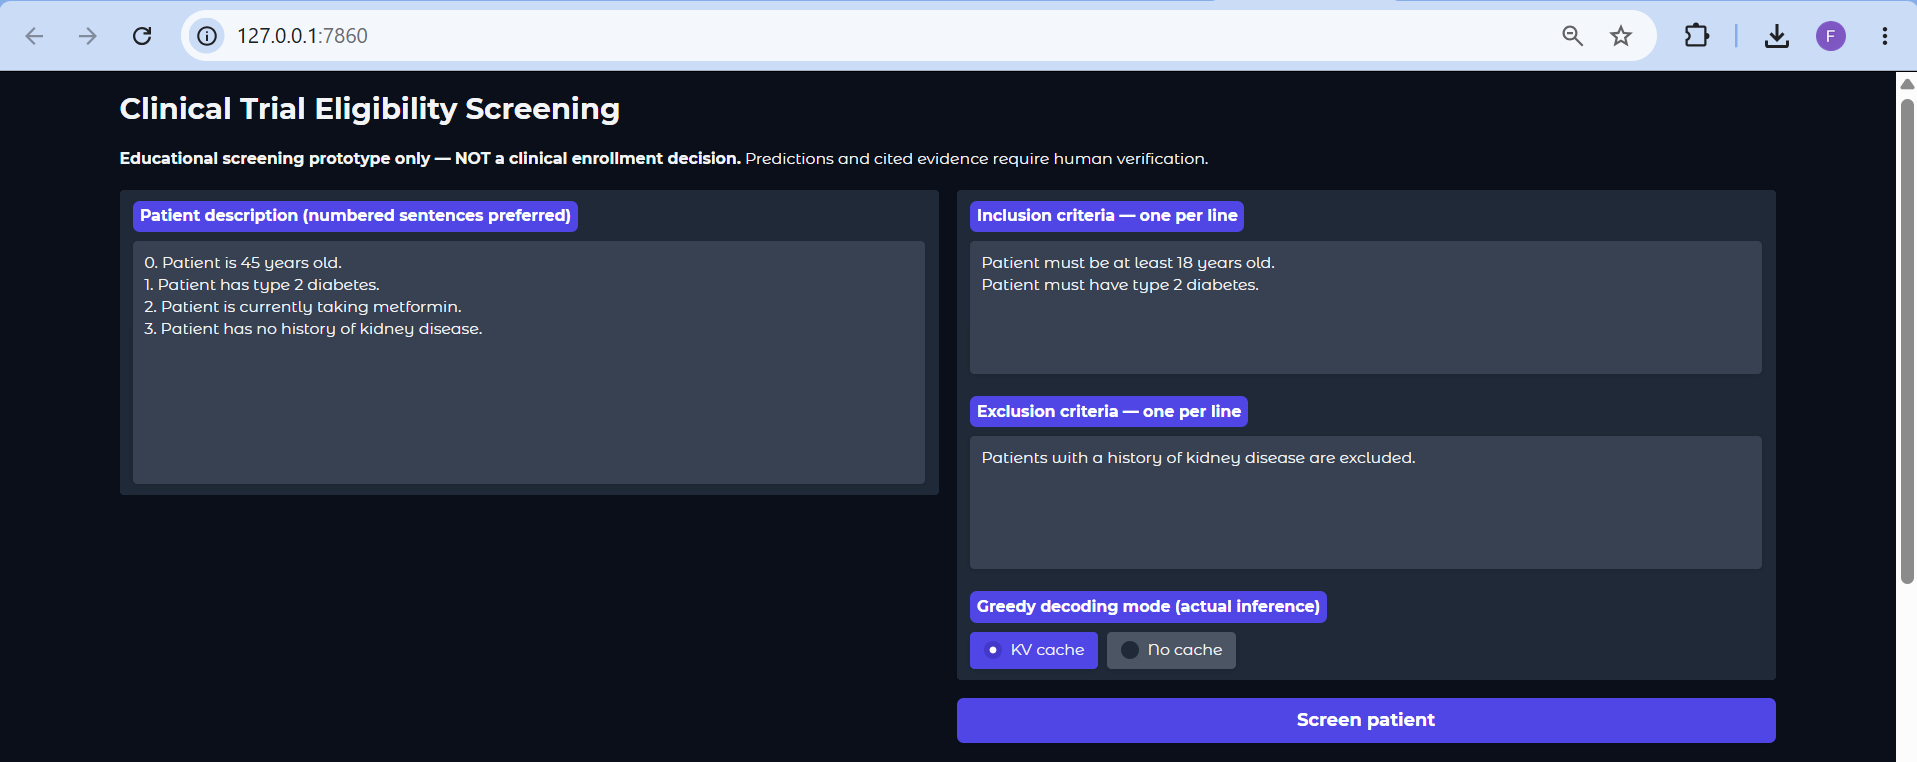
\includegraphics[width=0.91\textwidth]{figures/app_inputs.png}
\caption{Actual standalone Gradio interface showing numbered synthetic patient history, inclusion and exclusion criteria, KV-cache selection and the screening control. Screenshot provided from the running local application.}\label{fig:appinputs}
\end{figure*}
\begin{figure*}[!t]
\centering
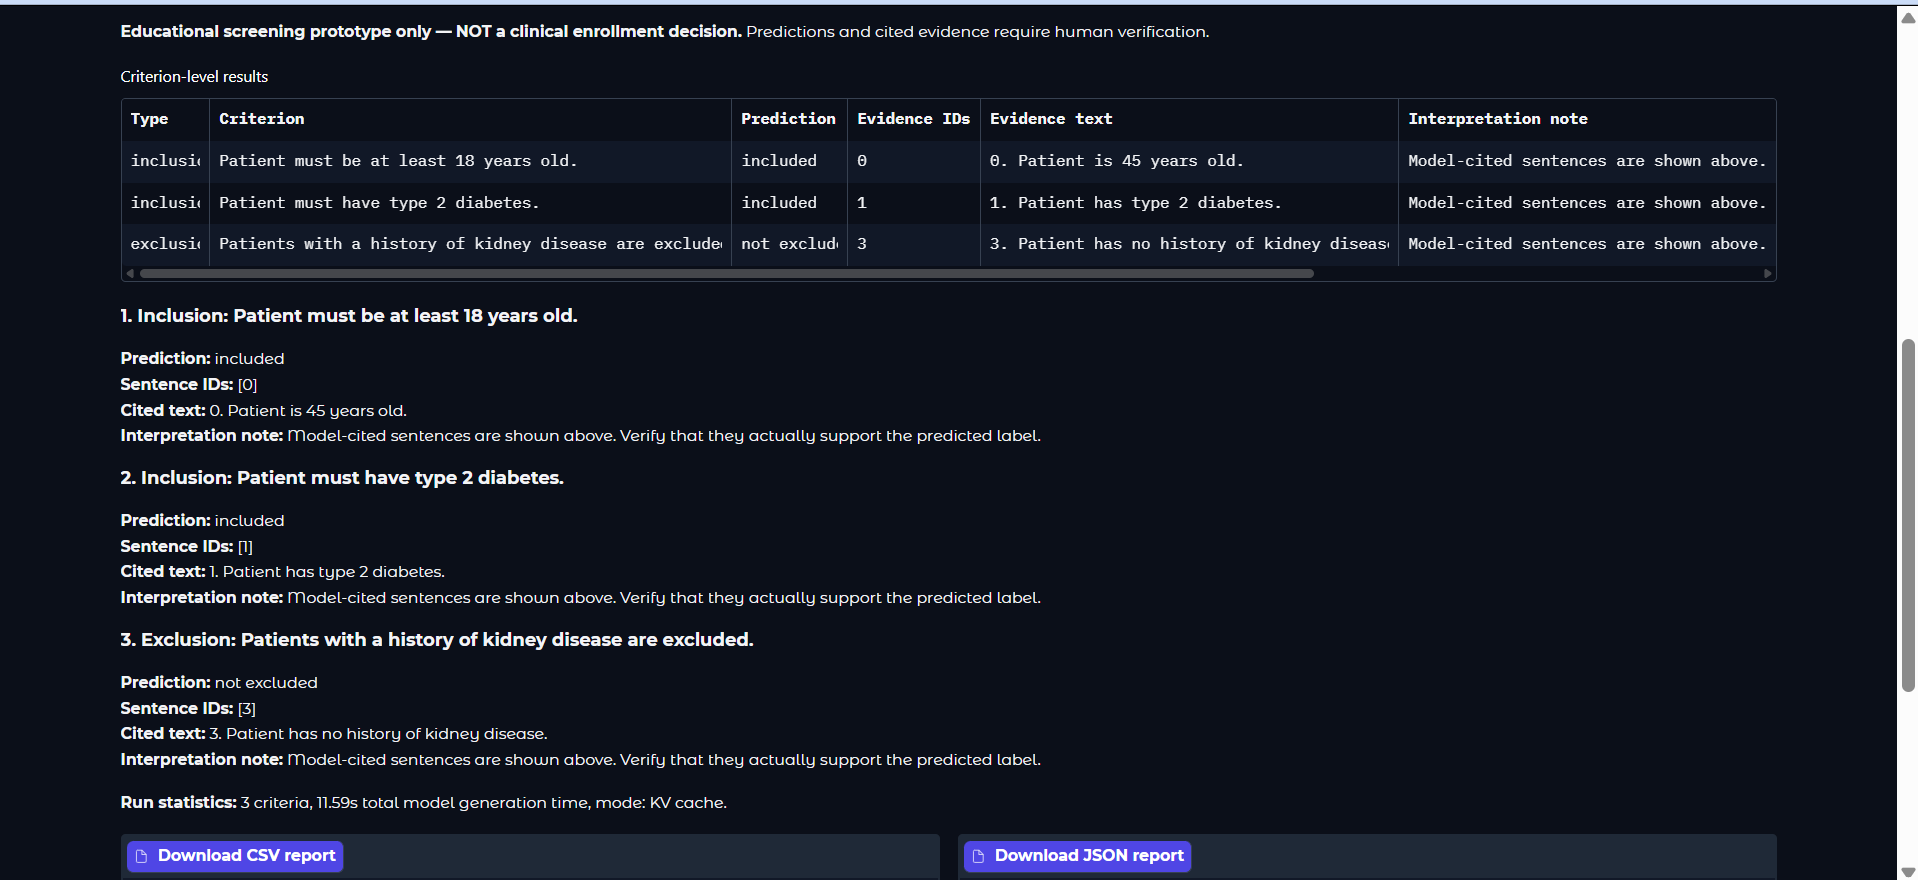
\includegraphics[width=0.91\textwidth]{figures/app_results.png}
\caption{Actual screening output for the kidney-disease example: the model identifies both inclusion criteria as satisfied and the documented absence of kidney disease as not excluded. Evidence sentences and CSV/JSON export controls are visible.}\label{fig:appresults}
\end{figure*}
\subsection{Two-case demonstration and observed error analysis}
Two synthetic patient scenarios are suitable for a transparent application demonstration. In the successful case, a 45-year-old patient has type 2 diabetes and explicitly reports no history of kidney disease. The two inclusion criteria (adult age and type 2 diabetes) were predicted \texttt{included} with evidence IDs 0 and 1; the kidney-disease exclusion was predicted \texttt{not excluded} with evidence ID 3. The saved application screenshot shows 11.59 seconds of cached generation for the three criteria. These labels and citations agree with the supplied narrative, although this single case is not a clinical validation study.

In the error case, a 52-year-old patient explicitly states in sentence 2 that they currently take metformin. The exclusion criterion says ``Patients currently taking metformin are excluded.'' The expected criterion label is \texttt{excluded} with supporting sentence ID 2. In repeated local tests, however, the model returned \texttt{not excluded} and cited sentence 1, which only establishes type 2 diabetes. This constitutes both a false negative for an exclusion condition and an unsupported citation. Because the application aggregates criterion-level predictions, it then displayed ``No model-identified disqualifying criteria'' despite the stated medication use. Both cached and uncached decoding produced the same wrong prediction, so the failure is not attributable to KV-cache optimization. A later prompt-definition modification did not reliably fix the error and once yielded an invalid label on an otherwise straightforward age criterion. The demonstration therefore preserves the original outputs and documents the limitation instead of hardcoding a correction.

These examples illustrate two separate evaluation dimensions: the successful case shows that labels and sentence-level evidence can align, while the metformin case shows that a fluent, structurally valid prediction can be clinically and evidentially wrong. Neither should be interpreted as a population-level estimate; quantitative test-set metrics are reported separately.

\section{Application Workflow, Reporting, and Safety}
The user supplies a patient description and one or more inclusion and exclusion criteria. The application validates that the inputs are nonempty, normalizes the patient description into numbered sentences, and constructs one criterion-specific prompt per criterion. The target model runs locally on CPU using the fine-tuned adapter; its JSON response is parsed into a six-category label and a list of evidence IDs. The UI displays the original criterion, predicted category, selected sentence IDs, corresponding patient sentences and measured inference latency. It also exports timestamped JSON and CSV reports.

\subsection{Preliminary aggregation is not ground truth}
The displayed overall outcome is a deterministic rule over criterion predictions, not a separately supervised trial-level model. A predicted \texttt{not included} or \texttt{excluded} can mark the patient as potentially ineligible; an insufficient-information result should prevent a confident positive conclusion. Because errors in criterion labels propagate into the aggregate, the UI must emphasize the model-derived nature of the result. In the local metformin test, the incorrect \texttt{not excluded} prediction caused a falsely reassuring aggregate. This is a concrete reason for prominently displaying uncertainty and source evidence.

\subsection{Provenance, privacy, and reproducibility}
Each exported report should record the model family, adapter identifier, decoding mode, timestamp and criterion-level outputs. A local browser address such as \texttt{127.0.0.1:7860} is not publicly reachable and must not be advertised as a deployed URL. The documented Windows launcher starts the local application using its virtual environment; on first use, the base checkpoint must be downloaded or made available in the local model cache. Patient descriptions can contain sensitive information. Local export directories should be excluded from public Git commits, and demonstration examples should be synthetic or otherwise cleared for sharing.

\subsection{Suggested acceptance tests}
Functional tests should cover a numbered narrative, an unnumbered narrative, multiple criteria, missing patient text, missing criteria, malformed model JSON, nonexistent evidence IDs, both decoding modes, CSV/JSON downloads and a fresh-process launch. The demonstrated successful tests establish the basic screening path and cached/uncached mode equivalence for one example; they do not establish that every edge case has already passed. Screenshots should be captured from the running application rather than synthesized for the report.

\section{Reproducibility and Deliverable Links}
\noindent\textbf{Source repository:} \url{https://github.com/FatimaShakir/GenAI-Assignment-2}.\\
\textbf{Public base model:} \url{https://huggingface.co/Qwen/Qwen2.5-0.5B-Instruct}.\\
\textbf{Alternative 1.5B base (not fine-tuned):} \url{https://huggingface.co/Qwen/Qwen2.5-1.5B-Instruct}.\\
\textbf{Fine-tuned LoRA adapter and draft model artifacts:} \url{https://drive.google.com/drive/folders/12UWSueNSTf1GRYghai724_B-3irobjgY?usp=sharing} (three downloadable ZIP archives: target LoRA, 12-layer draft, distilled draft adapter).\\
\textbf{Demonstration video:} \url{https://youtu.be/S7oah7-hhLw}.\\
\textbf{Browser app:} locally hosted; double-click \texttt{start\_app.bat}, then open \texttt{http://127.0.0.1:7860}.\\
The repository should include the completed Colab notebook, split manifest, evaluation JSON/CSV, figures, training and inference code, reproducibility instructions and this report's LaTeX source. The trained adapter and draft checkpoints should be hosted separately due to size. All download links must be accessible to the evaluator.
\section{Limitations, Ethics and Threats to Validity}
Patient-grouped test data contain only eight patients and uneven class frequencies. There are no gold \texttt{excluded} examples in the final test partition, so claims of reliable exclusion detection would be unsupported. Evidence retrieval is incomplete and citations can be semantically irrelevant even when sentence IDs exist. The baseline's invalid JSON rate conflates format compliance with semantic ability. CPU and GPU benchmarks use different hardware, sequence configurations and measurement protocols and must not be combined into a single speedup estimate. The attention implementation is not a fused kernel; the speculative draft has weak acceptance. No prospective clinical validation, calibration, privacy audit, or clinician adjudication was performed. Clinical text in exports should be handled as potentially sensitive and not committed publicly. The educational-use warning is mandatory.
\section{Conclusion}
Low-rank adaptation made a compact open-weight model produce well-formed criterion-level structured predictions and yielded 67.48\% held-out accuracy. However, minority labels and evidence attribution remain unreliable, and an observed metformin exclusion failure demonstrates the risk of aggregate false reassurance. Explicit KV caching preserved greedy outputs and offered modest GPU gains; tiled online softmax matched reference attention but incurred Python overhead; speculative decoding preserved tokens but regressed substantially because of poor draft acceptance. The local application makes these trade-offs inspectable while retaining human review as a necessary safeguard.
\section*{AI-Assistance Disclosure}
AI assistants were used for code drafting, debugging guidance, documentation organization and report preparation. Experimental numbers and plots in this paper were taken from the user's saved Colab outputs and local tests. AI-generated prose and code must be reviewed and validated by the student; no clinical judgment is delegated to the assistant.
\begin{thebibliography}{9}
\bibitem{attention} A. Vaswani \emph{et al.}, ``Attention Is All You Need,'' in \emph{NeurIPS}, 2017.
\bibitem{lora} E. J. Hu \emph{et al.}, ``LoRA: Low-Rank Adaptation of Large Language Models,'' in \emph{ICLR}, 2022.
\bibitem{flash} T. Dao \emph{et al.}, ``FlashAttention: Fast and Memory-Efficient Exact Attention with IO-Awareness,'' in \emph{NeurIPS}, 2022.
\bibitem{online} M. Milakov and N. Gimelshein, ``Online Normalizer Calculation for Softmax,'' arXiv:1805.02867, 2018.
\bibitem{speculative} Y. Leviathan, M. Kalman and Y. Matias, ``Fast Inference from Transformers via Speculative Decoding,'' in \emph{ICML}, 2023.
\bibitem{trialgpt} Q. Jin \emph{et al.}, ``TrialGPT: Matching Patients to Clinical Trials with Large Language Models,'' \emph{Nature Communications}, 2024.
\bibitem{qwen} A. Yang \emph{et al.}, ``Qwen2.5 Technical Report,'' arXiv:2412.15115, 2024.
\end{thebibliography}
\end{document}
